% ============================================================================
%  MASTER THESIS — Santiago Monsalve Bautista
%  Observatorio Astronómico Nacional (OAN) — Universidad Nacional de Colombia
%
%  Compilación:   latexmk  (desde la carpeta thesis/)   ->  ver .latexmkrc
%  Motor:         pdflatex + bibtex  (robusto, sin binarios extra)
%
%  NOTA IMPORTANTE sobre el formato:
%  La UNAL tiene una plantilla oficial de tesis (biblioteca / SINAB). Antes de
%  avanzar mucho, verificá con tu posgrado cuál es el formato vigente y, si
%  corresponde, reemplazá este \documentclass por el de esa plantilla. Este
%  esqueleto es genérico y funcional para empezar a escribir HOY; migrar el
%  contenido a la plantilla oficial después es trivial (los \chapter no cambian).
% ============================================================================
\documentclass[11pt,a4paper,oneside]{report}

% --- Codificación e idioma -------------------------------------------------
\usepackage[utf8]{inputenc}
\usepackage[T1]{fontenc}
\usepackage[spanish,es-noquoting]{babel}
 
% --- Matemática ------------------------------------------------------------
\usepackage{amsmath,amssymb,amsthm}
\usepackage{bm}            % negritas matemáticas (vectores/tensores)

% --- Figuras ---------------------------------------------------------------
\usepackage{graphicx}
\graphicspath{{../figures/}}   % figuras generadas por code/ viven acá
\usepackage{float}

% --- Bibliografía (natbib + bibtex: compila en cualquier lado) -------------
\usepackage[numbers,sort&compress]{natbib}
\bibliographystyle{unsrtnat}

% --- Márgenes y enlaces (hyperref SIEMPRE al final) ------------------------
\usepackage[margin=2.5cm]{geometry}
\usepackage[hidelinks]{hyperref}

% --- Comandos propios (agregá los tuyos acá) -------------------------------
\newcommand{\Rdot}{\dot{R}}
\newcommand{\Cc}{\mathcal{C}}
\newcommand{\rs}{r_{s}}
\renewcommand{\d}{\mathrm{d}}

% ============================================================================
\title{Simulation of matter into a \textit{Black Shell} configuration}
\author{Santiago Monsalve Bautista}
\date{\today}

\begin{document}

\maketitle

% --- Frontmatter -----------------------------------------------------------
% ============================================================================
% RESUMEN / ABSTRACT
% Objetivo: en un párrafo, qué hiciste y qué encontraste.
% Resultado que DEBE contener: la afirmación central de la tesis (ej. "se simuló
%   el colapso de una cáscara de polvo en los tres regímenes de Israel y se
%   caracterizó la condición de black shell en el límite de polvo (a=1/2)").
% Escribí esto AL FINAL, cuando sepas qué defendés. Por ahora, un placeholder.
% ============================================================================
\begin{abstract}
% TODO: resumen (½ página). Español + versión en inglés si el formato lo pide.
\end{abstract}


\tableofcontents

% --- Cuerpo ----------------------------------------------------------------
% ============================================================================
% CHAPTER 1 - INTRODUCTION 
% Objective: motive the problem and set reach.
% Result what must to have: 
%   · What is a black shell and why that matters (config. near the horizon).
%   · Why thin shell plus Israel-Darmois junction conditions) (vs. complete NR).
%   · General objective and the specific objectives (This define the minimum).
%   · Structure of the document (a paragraph).
% Criterion of reach: everything that do not worth for a an specific objective is
% candidate for a "future work"
% ============================================================================
\chapter{Introduction} \label{cap:introduccion}

% TODO: motivación — black shells, colapso de cáscaras, contexto.
% TODO: objetivo general.

Since the publication of the Einstein field equations the interest for a new object between the celestial bodies,a Black hole (BH). This object receives its name for the fact that it does not emit apparent radiation, what we know bout them come from the gravitational interaction. 

The gravitational collapse is one of the problems that unleash 

The develop of the \textit{Black Shell} model has been mark as a toy, something just to simplify the problem of the thermodynamics of a black hole (BH),but in the development of this so call toy where the inside of the "star" is flat metric the model has reveal an intricate dynamic that could tell something about the entropy of a BH. 

The dynamic of the shell has been studied \cite{israel1967} but there still conditions unexplored, like the introduction of a little bit of angular momentum. The study of the initial conditions is key to decode what lies behind the dynamics of the shell. 

The computational tool is ideal for this, for exploring initial conditions, Here is the general objective, develop a computational model to study the gravitational collapse of a shell of matter into a \textit{Black Shell} configuration with emphasis on the exploration of
initial conditions within the classical regime

% TODO: objetivos específicos (lista corta y realista). ESTO fija el alcance.


Study de collapse of a thin shell of dusk in its rapid phase using the Darmois-Israel formulation.

Analyse the effect that could have the different initial conditions upon the evolution of the system and the possible formation of a \textit{Black Shell}
          %hace falta el de comparación de modelos computacionales.

Identify the limitations of the model and discuss extensions to quantum effects,slow collapse or connections with thermodynamics of horizons.



% TODO: un párrafo mapeando los capítulos.
% en esta introducción debe ir una historia y un glosario para entender el propio articulo, en este deben ir los objetivos 
% ya la motivación. 

Since the publication of the Einstein field equations the interest for a new object between the celestial bodies,a Black hole (BH). This object receives its name for the fact that it does not emit apparent radiation, what we know bout them come from the gravitational interaction. 

The gravitational collapse is one of the problems that unleash 


% ============================================================================
% CAPÍTULO 2 — MARCO TEÓRICO
% Objetivo: derivar la ecuación de movimiento de la cáscara desde el formalismo.
% Resultado que DEBE contener:
%   · Condiciones de empalme de Israel (salto de la curvatura extrínseca).
%   · La ecuación maestra GENERAL en términos de f_±(R) — la fuente de verdad:
%       sqrt(Rdot^2 + f_-) - sqrt(Rdot^2 + f_+) = m/R
%   · La reducción a ODE para R(tau) via Birkhoff (por qué NO hace falta NR).
% Nota de honestidad para vos: acá va la derivación con los índices cuidados
%   (intrínseco vs. ambiente) — es donde históricamente aparecían los errores.
% Refs: Israel 1966; Poisson §3.7-3.8.
% ============================================================================
\chapter{Marco teórico: condiciones de empalme de Israel}
\label{cap:marco}

\section{Cáscaras delgadas y curvatura extrínseca}
% TODO: hipersuperficie tipo tiempo, n^mu espacelike, salto de K_ij.

\section{Ecuación de movimiento general}
\label{sec:eom-general}
% La condición de empalme para una cáscara de masa en reposo m(R):
\begin{equation}
    \sqrt{\Rdot^2 + f_-(R)} \;-\; \sqrt{\Rdot^2 + f_+(R)} \;=\; \frac{m(R)}{R}.
    \label{eq:maestra}
\end{equation}
% TODO: despejar Rdot^2 en general (resta de cuadrados) y comentar que este es
%   el núcleo que consumen integrador, benchmark y mapa.

\section{Reducción a una ecuación diferencial ordinaria}
% TODO: teorema de Birkhoff fija la geometría a ambos lados -> problema = ODE
%   para R(tau). Argumento explícito de por qué no se requiere NR 3+1.

% ============================================================================
% CAPÍTULO 3 — CÁSCARA DE POLVO
% Objetivo: especializar la ecuación general al caso polvo + Schwarzschild +
%   Minkowski y caracterizar TODA la familia de soluciones.
% Resultado que DEBE contener:
%   · La forma cerrada Rdot^2 = (a + b/2R)^2 - 1 como CASO PARTICULAR de la
%     ec. maestra (mostrar que sale de f_-=1, f_+=1-2M/R, m=b).
%   · La cantidad conservada C y su interpretación.
%   · Los tres regímenes (a<1, a=1, a>1) con R_max = b/(2(1-a)).
%   · El potencial efectivo V(R) y el retrato de fase (FIGURA del mapa).
%   · El locus black shell en el límite de polvo: a=1/2 (retorno en el horizonte)
%     CON el caveat: Rddot<0 siempre => no es equilibrio, es retorno momentáneo.
% Figura: initial_conditions_map.png (generada por code/).
% ============================================================================
\chapter{Collapse of a dusk shell}\label{cap:polvo}

\section{Ecuación de movimiento y cantidad conservada}
\begin{equation}
    \Cc \;\equiv\; 1 + \Rdot^2 - \left(a + \frac{b}{2R}\right)^2 \;=\; 0,
    \qquad a \equiv \frac{M}{b}.
    \label{eq:C}
\end{equation}
% TODO: derivar (\ref{eq:C}) desde (\ref{eq:maestra}); mostrar que es caso
%   particular. Rddot = -(b/2R^2)(a + b/2R) < 0.

\section{Los tres regímenes}
% TODO: tabla a<1 / a=1 / a>1, con R_max = b/(2(1-a)) y su significado físico.

\section{Potencial efectivo y retrato de fase}
\label{sec:mapa}
% TODO: V(R) = 1 - (a+b/2R)^2 ; región permitida/prohibida ; puntos de retorno.
\begin{figure}[H]
    \centering
    % 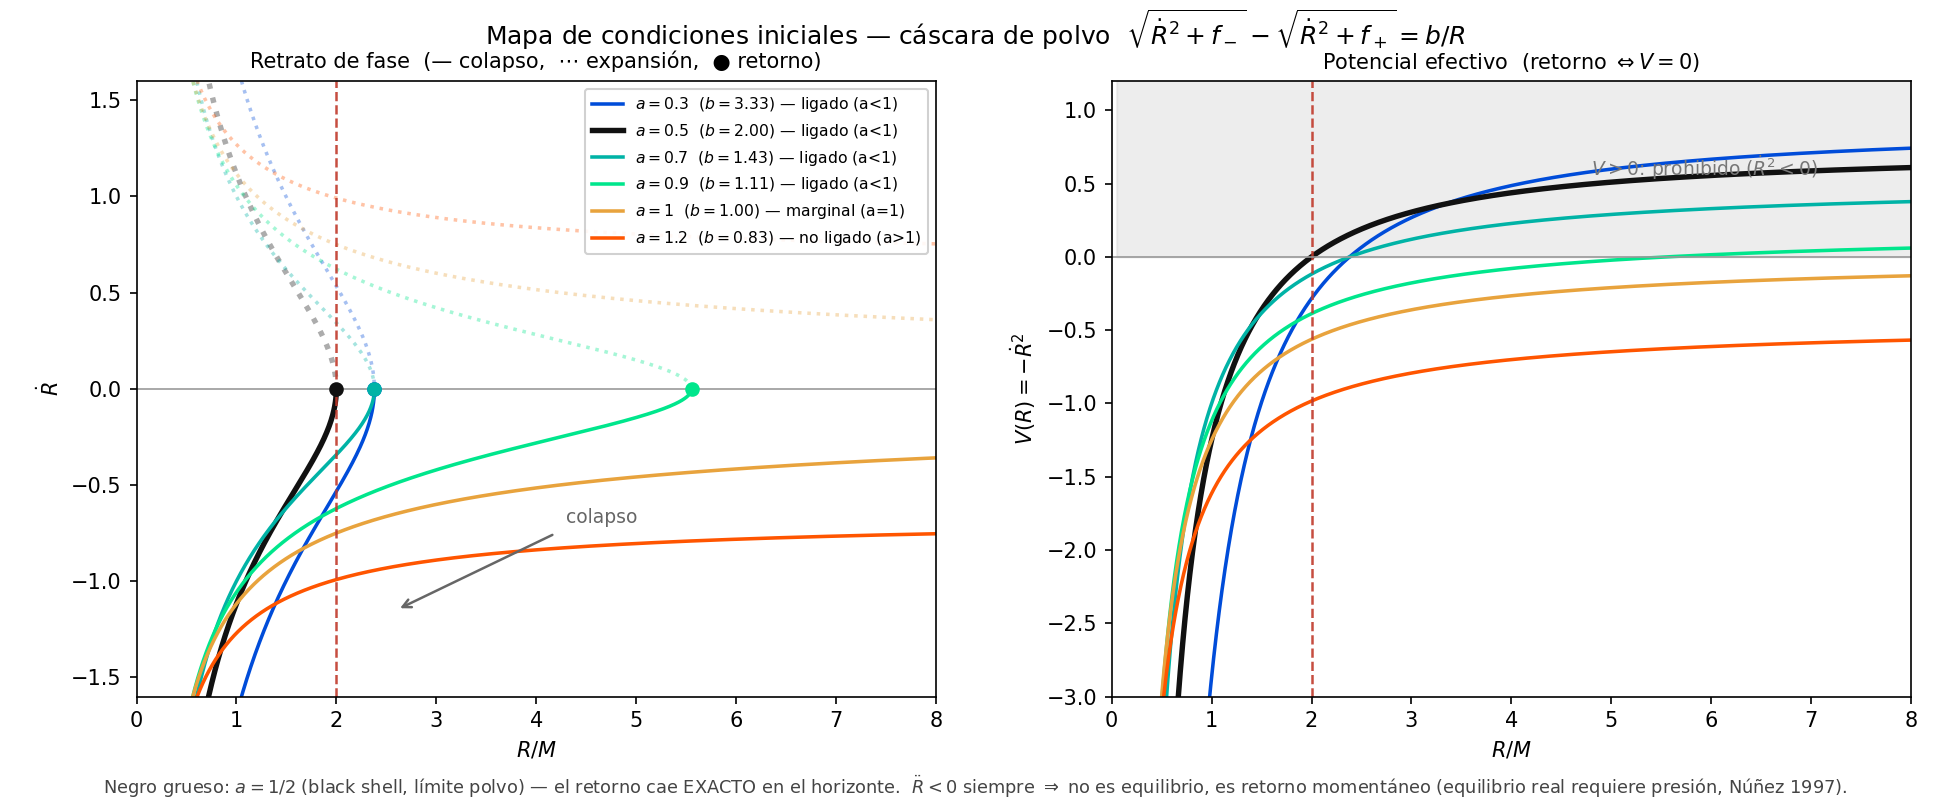
\includegraphics[width=\textwidth]{initial_conditions_map.png}
    \caption{Mapa de condiciones iniciales: retrato de fase $(R,\Rdot)$ y
             potencial efectivo para la familia de $a$. Los tres regímenes de
             Israel y el locus de black shell ($a=1/2$) en una sola vista.}
    \label{fig:mapa}
\end{figure}

\section{La condición de black shell en el límite de polvo}
% TODO: R_tp = r_s  =>  a = 1/2. Caveat de no-equilibrio (requiere presión).

% ============================================================================
% CAPÍTULO 4 — IMPLEMENTACIÓN NUMÉRICA
% Objetivo: describir el integrador propio y su validación.
% Resultado que DEBE contener:
%   · Arquitectura del código (spacetimes / shell / integrators / diagnostics).
%   · El RK4 de paso fijo (escrito a mano, por control y por ser formativo).
%   · El paso ADAPTATIVO por step-doubling: estimador de error local (~h^5),
%     controlador h_new = h·S·(tol/err)^{1/(p+1)}, rechazo-y-repite.
%     Motivación: en a>1 el ~99% de la dinámica está en el ~1% final cerca
%     del horizonte; el paso fijo desperdicia pasos en la región lenta.
%   · Validación: benchmark ExactParametric (a<1, a=1) y monitoreo de |C|.
%     OJO: el estimador de error del stepper y |C| son controles INDEPENDIENTES.
% CRITERIO DE ALCANCE: este capítulo justifica hacer o no el integrador a>1.
%   Si tus claims (cap. 5) no necesitan resultados a>1, esto se acota o se
%   reporta como limitación, no como bloqueante.
% ============================================================================
\chapter{Implementación numérica}
\label{cap:numerico}

\section{Arquitectura del simulador}
% TODO: diagrama de módulos y flujo de datos (ShellParams -> Runner -> ...).

\section{Integrador de Runge--Kutta de cuarto orden}
% TODO: esquema RK4; por qué implementación propia (control, formación).

\section{Paso adaptativo por duplicación de paso}
\label{sec:adaptativo}
% TODO: estimador de error local por step-doubling; controlador de paso;
%   tolerancia mixta atol + rtol·|y| por componente.

\section{Validación}
% TODO: comparación contra ExactParametric; drift de |C| (métrica exterior,
%   r>rs); por qué max_C_drift explota cerca de la singularidad (amplificación
%   numérica de b/2R, no error del integrador).

% ============================================================================
% CAPÍTULO 5 — RESULTADOS
% Objetivo: presentar lo que la tesis efectivamente demuestra.
% Resultado que DEBE contener (esto ES el núcleo defendible):
%   · Trayectorias de colapso R(tau) validadas en el régimen de polvo.
%   · El mapa de condiciones iniciales (retrato de fase + potencial).
%   · Clasificación de regímenes y cruce del horizonte.
%   · La condición de black shell (a=1/2) ilustrada sobre el mapa.
%   · (Si se hizo) resultados del régimen a>1 con el paso adaptativo.
% Regla: cada figura/afirmación acá debe trazarse a un objetivo del cap. 1.
%   Si una figura no sirve a un objetivo, no va en resultados.
% ============================================================================
\chapter{Resultados}
\label{cap:resultados}

\section{Colapso en el régimen de polvo}
% TODO.

\section{Mapa de condiciones iniciales}
% TODO: leer la Fig.~\ref{fig:mapa}; qué muestra que una trayectoria sola no.

\section{Cruce del horizonte y condición de black shell}
% TODO.

% ============================================================================
% CAPÍTULO 6 — EXTENSIONES Y TRABAJO FUTURO
% Objetivo: dejar planteadas, CON PROPIEDAD, las extensiones tratables.
% Contenido (según lo discutido, ordenado por costo real):
%   · Carga (Reissner-Nordström): cambio de f_+(R); la forma cerrada sobrevive
%     con coeficiente (b^2-Q^2)/b. Costo bajo. Refs: Kuchar 1968; Eid 2015.
%   · Rotación lenta O(Omega): NO rompe R(tau) a primer orden; agrega una
%     ecuación para omega(r). Arrastre perfecto en r_s (resultado on-theme
%     black shell). SECCIÓN REAL (decisión de Santiago). Refs: Hartle 1967;
%     Brill & Cohen 1966.
%   · Presión (Núñez): m(R) deja de ser constante; permite bounce y black
%     shell estático de verdad. Refs: Núñez 1996, 1997.
% NOTA: Kerr completo NO es una extensión — rompe el método (no hay Birkhoff).
%   Mencionar por qué queda fuera, para cerrar esa puerta con argumento.
% ============================================================================
\chapter{Extensions and future work}
\label{cap:extensiones}

\section{Cáscara cargada (Reissner--Nordström)}
% TODO: f_+ = 1 - 2M/R + Q^2/R^2 ; forma cerrada con (b^2-Q^2)/b (VERIFICAR
%   contra Kuchar 1968 / Eid 2015 el tratamiento de la autocarga).

\section{Rotación lenta y arrastre de marcos}
\label{sec:rotacion}
% TODO: expansión de Hartle O(Omega); ruptura confinada a g_{t phi};
%   omega_+(r)=2J/r^3 (Lense-Thirring); interior arrastrado (Brill-Cohen);
%   arrastre perfecto omega_- -> Omega cuando R -> r_s.

\section{Presión y black shell estático}
% TODO: generalización de m(R); conexión con bounce (Núñez).

\section{Por qué Kerr queda fuera}
% TODO: sin simetría esférica no hay Birkhoff; el shell deja de ser R(tau).

% ============================================================================
% CAPÍTULO 7 — CONCLUSIONES
% Objetivo: cerrar. LOGROS PRIMERO, después limitaciones (orden deliberado).
% Resultado que DEBE contener:
%   · Qué quedó demostrado (mapear 1:1 con los objetivos del cap. 1).
%   · Limitaciones honestas (régimen a>1, dust-only, sin presión/carga/spin).
%   · Trabajo futuro (puntero al cap. 6, sin repetir).
% ============================================================================
\chapter{Conclusions}
\label{cap:conclusiones}

\section{Logros}
% TODO: enumerar contra los objetivos específicos. Esto va primero.

\section{Limitaciones}
% TODO: honestas y acotadas. No te castigues; enunciá y seguí.

\section{Perspectivas}
% TODO: puntero corto al cap. 6.


% --- Apéndices -------------------------------------------------------------
\appendix
% ============================================================================
% APÉNDICE A — DERIVACIONES DETALLADAS
% Objetivo: descargar del cuerpo las cuentas largas pero necesarias.
% Candidatos:
%   · La cancelación u_alpha Du^alpha/dtau = 0 (contribuciones de f' y
%     Christoffel que se cancelan; la notación delta^2/delta s^2 de Israel).
%   · Álgebra completa del despeje de Rdot^2 desde la ec. maestra.
%   · Despeje del caso cargado (coeficiente (b^2-Q^2)/b).
% ============================================================================
\chapter{Derivaciones detalladas}
\label{ap:derivaciones}

\section{Despeje de $\Rdot^2$ desde la ecuación maestra}
% TODO.

\section{Cancelación de las correcciones de Christoffel}
% TODO.


% --- Bibliografía ----------------------------------------------------------
\bibliography{references}

\end{document}
